\setAuthor{}
\setRound{piirkonnavoor}
\setYear{2019}
\setNumber{G 2}
\setDifficulty{2}
\setTopic{TODO}

\prob{Peegel}
\begin{wrapfigure}[5]{r}{0.4\textwidth}
\vspace{-10pt}
	\begin{center}
		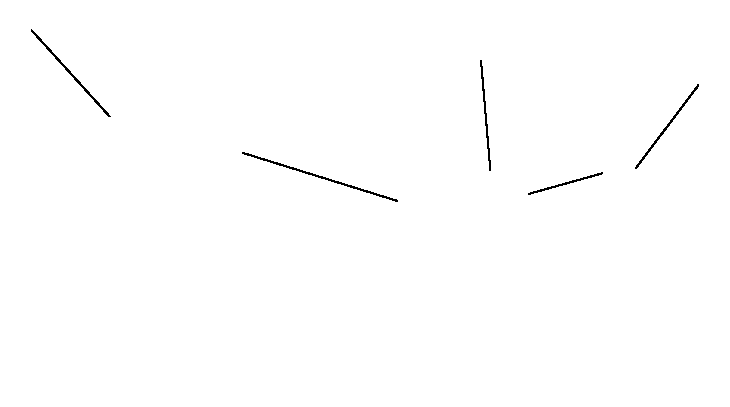
\includegraphics[width = 0.4\textwidth]{2019-v2g-02-yl.pdf}
	\end{center}
\end{wrapfigure}

Optilises skeemis (vt. joonis) on kujutatud kolme valguskiire viit fragmenti. Samuti on teada, et skeemis on tasapeegel, mis on joonise tasandiga risti. Rekonstrueerige peegli asukoht. Ülesanne lahendage lisalehel. 


\hint

\solu
Paneme tähele, et ükski kiirefragment ei ole teisega samal sirgel \pp{1}. See tähendab, et kõikide kiirefragmentide puhul on tegemist kas erinevate kiirtega või sama kiire fragmentidega enne ja pörast peegeldumist \pp{1}. Et kiiri on kokku ainult kolm, siis vähemalt kaks fragmenti peavad olema pärit samalt kiirelt, üks enne ning teine pärast peegeldumist \pp{1}. Kui me suudame kindlaks teha, millised on need kaks fragmendipaari, siis saame leida peegli asukoha kui kahe kiirepaari pikenduste lõikepunkte ühendava joone. Viis fragmenti annavad pikendades viis sirget, mis lõikuvad paarikaupa kümnes erinevas punktis. Pikendame kõiki kiiri lõikumisteni ja leiame need 10 lõikepunkti (9-10 lõikepunkti: \pp{1}; 8 või vähem lõikepunkti: \pp{0} punkti). Ühendame need 15 lõikepunktipaari, mida ühendav joon saab olla peegliks (st mis ei ole juba ühendatud fragmendipikendusega), joonega (punased jooned joonisel) (11-15 joont: \pp{1}; 10 või vähem joont: \pp{0}). Leiame punaste joonte hulgast sellise, mis sobib peegliks: joon moodustab vastavalt võrdsed nurgad lõikuvate kiirtega, (joonisel on võrdsed nurgad märgitud roheliste ja siniste kaarekestega ning peegli asukoht jämeda punase joonega) \pp{1}. 
\begin{center}
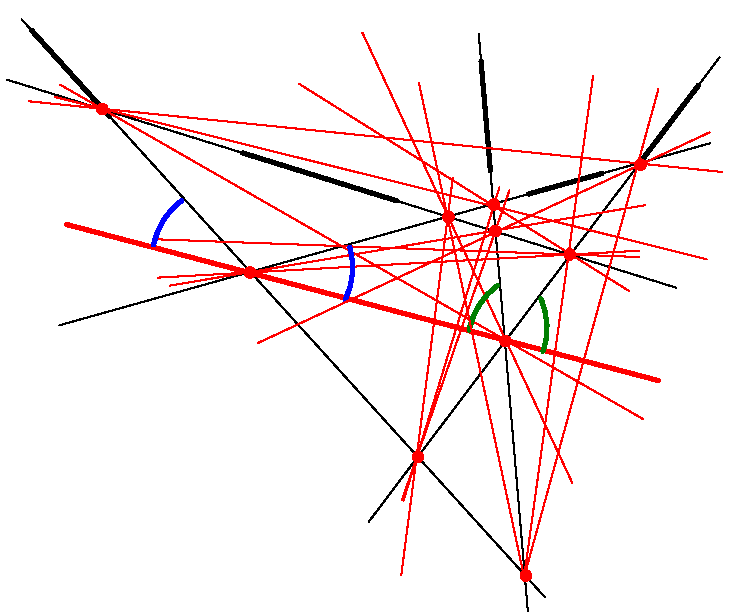
\includegraphics[scale=0.7]{2019-v2g-02-sol.pdf}
\end{center}
\probend